\documentclass{article}
\title{Implementazione di un modulo per il calcolo del Determinante in una Libreria Ibrida Cpu-Gpu}
\author{Povero Toninus}

\usepackage[cm]{fullpage}%set dei margini

\usepackage{xcolor} %pacchetto per cambiare il colore di simboli nei display math
\usepackage{graphicx}

\usepackage{amsmath}  %http://tex.stackexchange.com/questions/40028/highlight-elements-in-the-matrix
\usepackage{tikz}
\usetikzlibrary{arrows,matrix,positioning}

\usepackage[utf8x]{inputenc}%gli accenti

\usepackage{verbatim}%per i commenti
\usepackage{hyperref}% per i link a file



\begin{document}
\maketitle
\begin{abstract}

\end{abstract}

\section{Introduzione }
Nella prospettiva di un progetto piu' ampio della realizzazione di una libreria di calcolo numerico per l'algebra lineare ...
imbrida nel senso che si realizza una classe matrice....
Ogni volta che viene istanziata una variabile di tipo matrice vengono salvate due copie di essa, una sulla gpu e una sulla cpu..
%CORREGGI
.....

\begin{comment}
\section{Gli algoritmi per il calcolo del determinante}
Sostanzialmente se ne riconoscono 3 famiglie:
1) Algoritmi "naive" tipo laplace e liebniz: che si basano sul concetto di generare tutte le permutazioni di elementi di matrice appartententi a righe e colonne diverse e poi sommarli im base alla' parita' della permutazione.
2) Algoritmi di decomposizione : Consistono nel determinare delle matrici semplici il cui prodotto coincide con la matrice in esame. Come semplici si intende che abbiano un determinante noto e facilmente calcolabile.
3) Algoritmi di condensazione : Consistono nell'applicazione consecutiva di una trasformazione (non lineare) della matrice che la trasforma in una matrice quadrata di ordine piu' basso. se l'abbassamento dell'ordine e' da M(n,n) a M(n-1,n-1) saranno ovviamente necessari n applicazioni consecutive. Il cuore di questa classe di algoritmi e' di applicarli finche' non si trasforma la matrice iniziale in uno scalare, la trasformazione viene scelta in modo che questo scalare coincida con il determinante della matrice.
%CORREGGI
......
\end{comment}

\section{Gli Algoritmi di Condensazione}
Sono una classe di algoritmi nata specificatamente per il calcolo del determinante di matrici quadrate.
L'idea chiave e' la seguente: si identifica una trasformazione $$\mbox{T}: A \in \mbox{ Mat}(n,n) \longmapsto B \in \mbox{ Mat}(n-1,n-1)$$
tale per cui esista uno scalare $\alpha_{A}$, in generale dipendente dalla matrice di partenza, tale che:
\begin{displaymath}
\mbox{det}(A) = \alpha_{A} \cdot \mbox{det}(B)
\end{displaymath}
Ammettendo che l'operatore T sia applicabile $n-1$ volte sulla matrice quadrata $A$ di ordine $n$  e definendo:
\begin{displaymath}
	A_{0} = A \qquad \mbox{T}(A_{k})= A_{k+1} \qquad \mbox{det}\big(A_{k}\big) =  \alpha_{k}\mbox{det}(A_{k+1} )
\end{displaymath}
Si conclude banalmente che 
\begin{equation}
	\mbox{det}\big(A\big) = \prod_{k=0}^{n-1} \alpha_{k}
\end{equation}

\subsection{La formula di Dodgson}
Il primo algoritmo di questo tipo e' stato introdotto da C. L. Dodgson \cite{Carroll}, noto come Lewis Carroll, nel 1866.
Gli elementi della matrice trasformata $B = \mbox{T}_{D}(A)$ sono definiti come segue:
\begin{equation}\label{eq:Dodgson}
b_{i,j} =
\left| \begin{array}{cc} a_{0,0} & a_{0,j+1}  \\ a_{i+1 , 0} & a_{i+1 , j+1}  \end{array} \right| 
\end{equation}
Praticamente tale metodo rimpiazza gli elementi della sottomatrice ottenuta privando $A$ della prima riga e della prima colonna con con il determinante della matrice 2x2 costituita dal primo elemento in alto a sinistra $a_{00}$ ,il primo valore nella colonna dell'elemento, il primo valore nella riga dell'elemento e il valore dell'elemento stesso da sostituire.
Per esempio la riduzione di una matrice 3x3 risulterebbe:
\begin{displaymath}
	A =
\left[ \begin{array}{ccc} \ast & \ast & \ast  \\ \ast & (a_{00}a_{11} - a_{01}a_{10}) & (a_{00}a_{12} - a_{02}a_{10}) \\ \ast & (a_{00}a_{21} - a_{01}a_{20}) & (a_{00}a_{22} - a_{02}a_{20})  \end{array} \right] 
	=
\left[ \begin{array}{cc} b_{00} & b_{01} \\ b_{10} & b_{11} \end{array} \right]
	=
	B
\end{displaymath}
Si dimostra per induzione che per questa trasformazione vale la seguente  equazione di condensazione del determinante:
\begin{equation}
 \mbox{det}\big(A\big) = \dfrac{\mbox{det}\big(B\big)}{a_{00}^{n-2}}
\end{equation}

Prima di indagare ulteriormente sull'efficienza di questo metodo e' necessario osservare che questo algoritmo soffre di un importante limitazione algebrica: se il primo elemento della matrice e' nullo la condensazione non puo' avvenire.

E' evidente che nel procedimento di Dogdson l'elemento $a_{00}$ riveste il ruolo di "Pivot" (nel senso di elemento cardine per il passo di condensazione) pertanto e' necessario introdurre qualche forma di prescrizione (o "pivoting") per scegliere un diverso elemento su cui basare la condensazione.

\subsection{La formula di Salem-Said}
Rappresenta il più' naturale miglioramento del metodo precedente: come pivot non viene preso il primo elemento della prima riga ma il primo elemento non nullo. In questo modo la successione degli step di condensazione puo' proseguire senza intoppi a meno che la prima riga della matrice non sia completamente nulla, quindi singolare.
\newline
Sia $a_{0l}$ il pivot, in questo caso la matrice $ \mbox{T}_{\small SS}\big(B\big)=(b_{ij})$ prodotta dallo step di condensazione risulterebbe:

	\begin{equation}
		b_{i,j}= 
		\begin{cases} 
			\left| \begin{array}{cc} a_{0,l} & a_{0,j+1}  \\ a_{i+1 , l} & a_{i+1 , j+1}  \end{array} \right| & \mbox{ se } j \geq l \\ 
			 & \\
			\left| \begin{array}{cc} a_{0,j} & a_{0,l}  \\ a_{i+1 , j} & a_{i+1 , l}  \end{array} \right| = -a_{0,l} a_{i+1 , j}, & \mbox{ se } j<l
		\end{cases}
	\end{equation}
Nel loro articolo \cite{arx:SalemSaid} gli autori dimostrano che in questo caso vale un'equazione di condensazione simile a quella precedente:
	\begin{equation}
		 \mbox{det}\big(A\big) = \dfrac{\mbox{det}\big(B\big)}{a_{0,l}^{n-2}}
	\end{equation}
In sostanza il calcolo del determinante con il metodo di Salem e Said si riduce al calcolo del prodotto di potenze degli inversi dei pivot.


\subsubsection{Complessità Algebrica}
Il numero di operazioni aritmetiche necessarie per completare l'esecuzione dell'algoritmo precedente e facilmente stimabile:
\begin{itemize}
\item \textit{Pivoting}: per ogni step di condensazione richiede al più $n$ letture per trovare il primo elemento non nullo nella prima linea

\item \textit{Singolo step di Condensazione}: per calcolare ogni elemento della matrice $B$ è necessario il calcolo di 2 prodotti e di 1 sottrazione. Quindi sono richieste $3(n-1)^{2}$ operazioni.

\item \textit{Condensazione}: per calcolare il determinante sono necessari $(n-2)$ step di pivoting e condensazione. 

\end{itemize}
In conclusione il costo complessivo per calcolare il determinante con un algoritmo di condensazione risulta dell'ordine di $O(n^{3})$.
Tali algoritmi risultano molto più efficienti rispetto agli algoritmi di Laplace e Liebniz, basati sulla definizione esplicita di determinante, che richiedono un numero di operazioni dell'ordine di $O(n!)$ . 


\subsubsection{Stabilità numerica}
L'implementazione computazionale di un algoritmo di questo tipo presenta comunque un'importante limitazione di stabilità numerica, più precisamente dopo pochi passi di condensazioni c'è un elevato rischio di underflow o overflow, ovvero il tipo di struttura dati scelta per immagazzinare in memoria il valore degli elementi della matrice condensata potrebbe avere delle limitazioni troppo restrittive riguardo al più piccolo e più grande numero rappresentabile .
Il problema può essere essere evidenziato come segue:
sia $S = <A>$ la "dimensione caratteristica" o "taglia" della matrice $A$ da condensare, non esiste un modo formale per definire questo valore ma lo si può ad esempio prendere come la media dei valori assoluti di tutti gli elementi della matrice.
E' evidente che dopo uno step di condensazione la taglia della matrice $B$ risulterà essere:
\begin{equation}
<B> = <(a_{\ast}a_{\ast} -a_{\ast}a_{\ast})>  \simeq S^{2}
\end{equation}
Pertanto dopo $n$ condensazioni la taglia crescerà ( o convergerà verso lo 0 in caso di $S<1$) molto rapidamente, tale andamento si può stimare essere:
\begin{equation}
<B_{n}> = \big( S \big) ^{2n}
\end{equation}
La cosa in realtà non sorprende, considerando la definizione di determinante (come sommatoria di numerose permutazioni) è chiaro che l'ordine di grandezza di det$(A)$ cresca come la potenza n-sima della taglia. In questo caso però Il problema si palesa molto prima di essersi avvicinati alla valore del determinante, il possibile under/over - flow  si può presentare già dai primi passi di condensazione.

\subsection{Una possibile modifica all'algoritmo di Salem-Said}
Considerando la specifica classe di matrici su cui si vuole implementare questo algoritmo (grandi, dense, con valori degli elementi distribuiti uniformemente tra un valore minimo e un massimo) l'algoritmo di Salem-Said non è direttamente applicabile per via del problema di stabilità numerica evidenziato in precedenza.
Notando che ogni routine di Condensazione, derivata dagli algoritmi precedenti, è in generale costituita da un ciclo che ripete $n-1$ volte le seguenti operazioni:
\begin{enumerate}
\item Viene scorsa la prima riga , o al limite l'intera matrice, per determinare l'elemento di Pivot.
\item Viene Trasformata la matrice $ A \mapsto A'$
\item Viene Condensata la matrice trasformata
\end{enumerate}
che determina una lista di $n$ valori, ottenuti a partire dai $n-1$ pivot più il singolo elemento che si ottiene dopo tutte le condensazioni, il cui prodotto coincide con il determinante.

Per ovviare al problema dell'overflow, o meglio per tenerlo sotto controllo limitando questo rischio solo al calcolo della produttoria finale, viene proposta una modifica ai primi 2 punti del ciclo.

\begin{enumerate}
\item \textbf{Pivoting}: viene scelto come pivot l'elemento in modulo più grande dell'ultima riga della matrice e viene salvato il valore $p$ del pivot.
\item \textbf{Trasformazione}: viene divisa l'ultima riga per il valore di pivot e ,se necessario, viene scambiata la colonna in cui si trova l'elemento di pivot con l'ultima colonna della matrice e cambiato il segno di $p$ in modo da tener conto che la matrice iniziale è stata moltiplicata per una di permutazione.
\item \textbf{Condensazione}: siccome a questo punto l'elemento di pivot della matrice da condensare si trova nell'angolo in basso a destra, la formula di condensazione assume un'espressione particolarmente semplice:
\begin{equation}\label{eq:CondMia}
b_{i,j} =
\left| \begin{array}{cc} a_{i,j}' & a_{i , n-1}'  \\ a_{n-1 , j}' & a_{n-1,n-1}'  \end{array} \right|  \qquad \forall i,j \in [0, n-2]
\end{equation}
dove $a_{n-1,n-1}' $ coincide con il valore dell'elemento di pivot trovato nel punto 1).

\end{enumerate}
Alla fine di questo processo il valore del determinante si ottiene dalla produttoria di tutti i pivot trovati con la routine precedente.
Questo deriva dalla semplice identità algebrica
\begin{displaymath}
	\mbox{det}\big(A\big) = \left| 
		\left[ \begin{array}{ccc}
			1 & 0 & \cdots \\
			0 & \ddots & \\
			\vdots & &p
		\end{array} \right]
		\left[ \begin{array}{ccc}
			1 & 0 & \cdots \\
			0 & \ddots & \\
			\vdots & &\frac{1}{p}
		\end{array} \right]
		  A\: \right|
		 	=
	   p \;	\mbox{det}\big(A'\big)
\end{displaymath}
e dall'equazione di condensazione di Salem Said per cui il determinante della matrice condensata coincide con quello della matrice di partenza nel caso che il pivot sia uguale ad 1 ovvero:
\begin{displaymath}
\mbox{det}\big(A'\big) = \mbox{det}\big(B\big)
\end{displaymath}
\newline
Il vantaggio principale di questo pivot deriva dal fatto che la taglia della matrice condensata rimane dello stesso ordine di grandezza di quello di partenza, infatti considerando l'equazione \ref{eq:CondMia} e che il pivot di $A'$ è  a seguito della divisione per il pivot $ a_{n-1,n-1}'=1$ risulta che:
\begin{displaymath}
<B> = <(a_{\ast}' 1 -\alpha a_{\ast}')>  \simeq S - \alpha S \simeq S
\end{displaymath}
dove $\alpha$ e il rapporto tra un elemento della riga del pivot e il valore del pivot, ovvero $-1<\alpha < 1$.

Il motivo dello swap di colonne e della scelta dell'ultima riga della matrice come riga di pivot ha invece una motivazione puramente computazionale che verrà discussa nei seguenti paragrafi.

\section{Implentazione dell' Algoritmo su Cpu}
L'implementazione dell' algoritmo precedente come una routine sequenziale sulla cpu è piuttosto immediato.
Dopo aver trovato il pivot e aver scambiato la sua colonna con l'ultima,  viene eseguito un ciclo for che scorre tutta la matrice da sinistra a destra e dall'alto verso il basso. 
Questo schema di lettura è suggerito dal criterio che ha la classe \textit{Matrice} di immagazzinare in memoria la matrice come un array 1D.
Ad ogni passo vengono letti i 2 valori sulla riga e colonna del pivot, il valore da modificare e viene riscritto immediatamente il risultato sull'array originale.
Per esempio per una matrice 3x3 i risultati delle 2 condensazioni successivi verrebbero riscritte nel seguente modo:

\begin{displaymath}
\left[ \begin{array}{ccc} a_{00} & a_{01} & a_{02} \\ a_{10} & a_{11} & a_{12} \\ a_{20} & a_{21} & a_{22}  \end{array} \right] 
\mapsto
\left[ \begin{array}{ccc} \color{blue}b_{00} & \color{blue}b_{01} & \color{blue}b_{10} \\ \color{blue}b_{11} & a_{11} & a_{12} \\ a_{20} & a_{21} & a_{22}  \end{array} \right] 
\mapsto
\left[ \begin{array}{ccc} \color{green}D & \color{blue}b_{01} & \color{blue}b_{10} \\ \color{blue}b_{11} & a_{11} & a_{12} \\ a_{20} & a_{21} & a_{22}  \end{array} \right]
\end{displaymath}
Ad ogni passo del ciclo pivoting - trasformazione - condensazione viene salvato in memoria il pivot. 
Come già detto per il calcolo del determinante è necesarrio calcolare la produttoria di questi valori, per matrici grandi è necessario immagazzinare questi valori in una struct apposta che memorizzi separatamente la mantissa e l'esponente del numero in esame.

L'aver posto il pivot nell'angolo in basso a destra dà la garanzia che ogni volta che si tenterà di aggiornare un sito della matrice al valore condensato tutti i dati necessari siano disponibili e non sovrascritti. Grazie a questo accorgimento è possibile allocare un solo array in memoria e non è necessario disporre di un secondo array su cui salvare il risultato della condensazione.
E' da notare che alla fine di questo processo le informazioni sulle componenti della matrice iniziale sono state perse ma è possibile sfruttare la peculiarità della classe ibrida che conserva sulla memoria global della gpu una copia della matrice in esame.


\section{Implementazione dell'Algoritmo su Gpu}
Come prima, la routine viene sostanzialmente eseguita in 3 passi, ad ognuno di essi corrisponderà uno specifico kernel CUDA che agirà esclusivamente sulla copia gpu della matrice considerata.
Sono da notare alcune differenze:

La prima risiede nello spiccato utilizzo della struttura ibrida della classe. 
Questo interviene, in primo luogo, nel calcolo della produttoria finale, che viene eseguita esclusivamente dall'host.
Il motivo di questa scelta è la superiore efficienza della cpu nel calcolo di questo tipo di operazioni su array non troppo grandi ( il numero di pivot coincide con l'ordine della matrice) e nella maggiore affidabilità nell'utilizzare strutture dati ( Classi c++) personalizzate , in questo caso la classe per i numeri grandi.
Affinchè l'host possa eseguire questo calcolo è necessario che tutta la lista dei pivot venga copiata dalla memoria global al host.
\newline
Invece di copiare la lista dei pivot in una sola volta alla fine di tutto il calcolo viene passato un singolo valore ogni volta che viene eseguito il pivonting.
La presenza sulla memoria host di questo dato permette di trarne vantaggio anche per l'operazione di divisione dell'ultima riga per il pivot.
Infatti dividere gli elementi di un array presente sulla memoria global della scheda per il valore di una specifica entry soffrirebbe di un elevato traffico in lettura, dovuto al fatto che tutti i thread dovrebbero leggere almeno una volta sulla cella di memoria contenente il dividendo. Siccome questa operazione non può essere eseguita in parallello i thread saranno forzati ad agire in sequenza  determinando un evidente perdita di parallelismo.
Ci sono 2 possibili soluzioni per ovviare a questo problema, il primo è passare il dividendo per valore come argomento del kernel, la seconda è sfruttare la memoria costant fornita da CUDA che assicura una lettura molto veloce da parte dei thread del kernel ma che in scrittura è accessibile solo dall'host.

La seconda è più sostanziale e riguarda il procedimento di scrittura in memoria degli elementi della matrice condensata.
In questo caso non è possibile sfruttare il pattern di lettura - scrittura utilizzato per l'algoritmo Cpu perchè il non perfetto parallelismo tra i thread non assicura che nel momento di scrivere sulla matrice originale gli elementi da leggere non siano già stati modificati da altri thread,
La soluzione più semplice per superare questo problema è quello di allocare sulla memoria global della gpu un array adatto a contenere i dati della matrice risultato della condensazione. Alla fine dello step sarà sufficiente disallocare la memoria relativa alla matrice vecchia e sostituire il valore del puntatore alla copia gpu, presente tra gli attributi della classe, con l'indirizzo della matrice trasformata.

Detto questo l'operazione di scambio della colonna del pivot con la colonna più esterna potrebbe sembrare superflua. Invece questo accorgimento si rivela utile per preservare la coelescenza degli indirizzi. In questo modo se tutti i thread di un blocco scriveranno elementi contigui di una riga della matrice $B$ è garantito che leggeranno celle contigue anche nella matrice di partenza $A$.

\subsection{Kernel di condensazione}
Del Kernel che esegue lo step di condensazione, su una matrice precedentemente arrangiata con il termine di pivot in basso a destra, sono state realizzate cinque versioni, il codice è presente in forma commentata in \url{ProgettoFinale/KernelTest/condensation_tentative.cuh}.

Tutti questi kernel sono stati pensati per  essere lanciati con una griglia 2d di blocchi 1d, il numero di thread ottimale deve essere tale che la griglia sia sufficientemente larga da coprire almeno una volta l'intera larghezza della matrice.
Questa disposizione fa emergere immediatamente il problema che tutti i thread che dovranno di calcolare simultaneamente la riga $i$ della matrice condensata $B$ tenterenno di leggere contemporaneamente il valore $a_{i,n-1}$ nella colonna del pivot determinando un collo di bottiglia simile a quello che si presenta quando si cerca di dividere  una riga per il pivot.

Visto che l'obbiettivo è trattare matrici molto grandi, qualsiasi via che sfrutti la memoria constant o il passaggio dei valori per argomento non è percorribile in questo caso.
L'approccio che si è dimostrato migliore è stato quello di sfruttare la memoria texture dell'architettura CUDA. Se prima di ogni passaggio di condensazione si procede ad un\emph{bind} dell'array degli elementi di matrice come un texture monodimensionale si garantisce una notevole velocizzazione dei thread nel leggere tutti i valori necessari al calcolo del singolo elemento di $B$ oltre che l'elemento di maggiore traffico.

Con questo accorgimento e con la disposizione della griglia e dei blocchi detta prima si garantisce, oltre ad un efficiente pattern di lettura nella memoria, anche la coalescenza di indirizzi visto che tutti i thread nel blocco eseguono le stesse quattro operazioni su celle contigue:
\begin{enumerate}
\item I thread contigui del blocco leggono celle contigue sulla memoria texture lineare contenente $A$
\item I thread del blocco leggono tutti lo stesso elemento sulla colonna del pivot
\item i thread contigui del blocco leggono celle contigue sulla riga contenente il pivot (anche questa si trova sulla memoria texture contenente $A$)
\item ogni thread calcola l'elemento di $B$ e lo scrive su celle di memoria contigue.
\end{enumerate}

E' da notare però che la dimensione massima della memoria $bindabile$ come texture non è illimitata e dipende delle specifiche di ogni dispositivo Nvidia.

Per questo è stato implementato anche un kernel che fa un utilizzo inferiore della memoria texture. In questo specifico caso viene fatta una copia della colonna contenente il pivot su un secondo array (quindi messi anch'essi in linea) che viene subito dopo \emph{bindato} come texture per garantire una lettura più efficiente e sulla stessa cella di memoria. In questo caso la memoria texture occuperà solo $n$ celle invece che $n^{2}$.


\section{Conclusioni}
Oltre ai programmi necessari a testare il corretto funzionamento degli algoritmi sono state effettuate delle prove di performance per mettere a confronto il tempo necessario al calcolo della lista dei pivot impiegato dall'algoritmo cpu e dai due algoritmi gpu discussi nel precedente paragrafo ( come "best" si intende il metodo che sfrutta il bind a texture dell'intera matrice).
\begin{figure}[ht!]
	\centering
	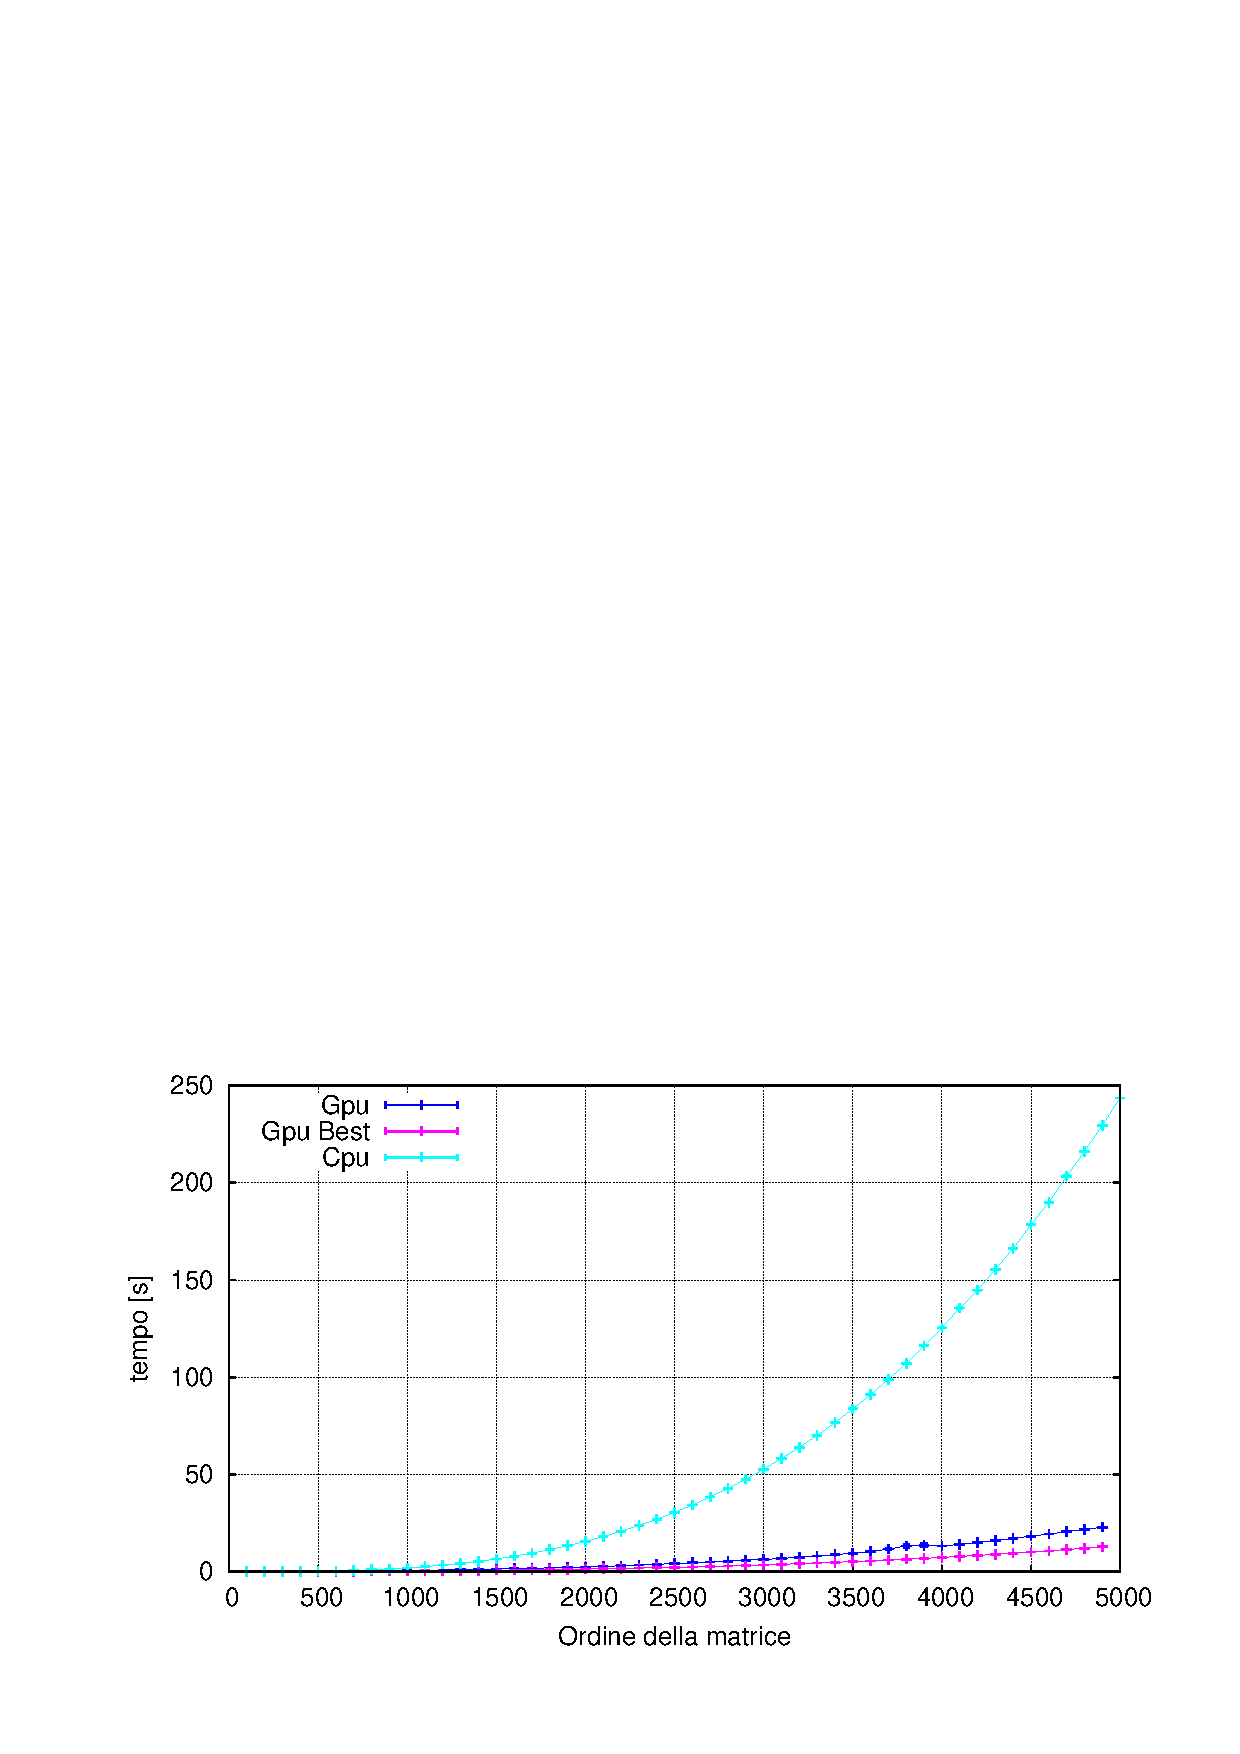
\includegraphics[width=180mm]{TimevsN.pdf}
	\caption{Confronto tempo d'esecuzione vs Taglia della matrice}
	\label{TimevsN}
\end{figure}
Dal grafico \ref{TimevsN} è evidente senza alcun dubbio come l'algoritmo parallelizzato con CUDA sia estremamente più veloce rispetto alla Cpu già  a partire dalle matrici di ordine 1000. E' necessario notare però che le API di CUDA non permettono di allocare array di celle contigue nella memoria global oltre una certa dimensione, questo determina un limite alla dimensione massima delle matrici considerabili. In questi test non si è andato oltre i $\tilde 10^{8}$ elementi di tipo \emph{float}.
\begin{figure}[ht!]
	\centering
	\caption{Confronto tempo d'esecuzione vs Taglia della matrice (zoom)}
	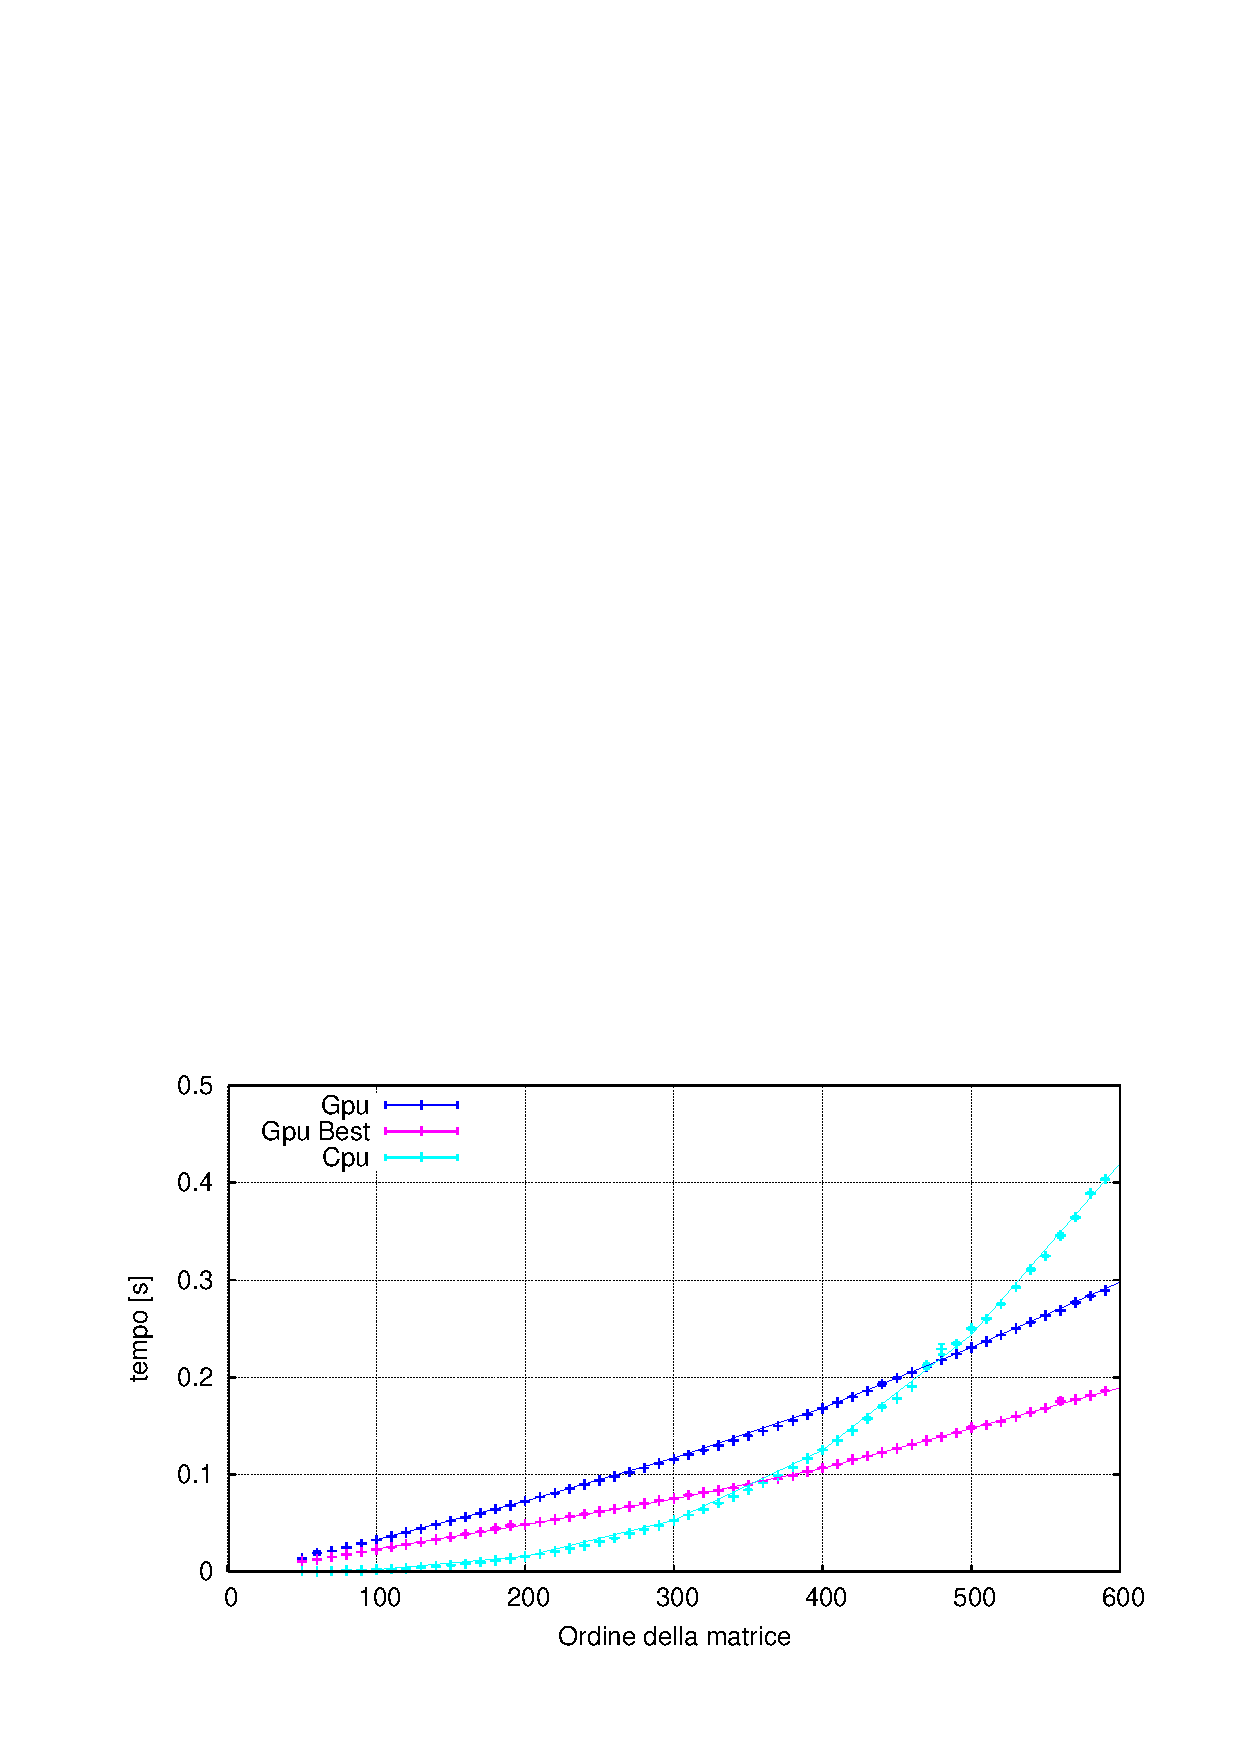
\includegraphics[width=180mm]{TimevsN_Zoom.pdf}
	\label{Zoom}
\end{figure}
Osservando invece il grafico \ref{Zoom} si nota che la situazioni è invertita quando si considerano matrici più piccole, per matrici fino all'ordine $n = 350$ l'algoritmo classico si dimostra più perfomante. Questo non è sorprendente, preso singolarmente il singolo thread dell'architettura CUDA non raggiunge la velocità del singolo thread della cpu.
La scheda video riesce ad eccellere nel momento in cui vengono realizzati dei kernel in grado di distribuire il calcolo uniformemente tra un eleveta numero di thread.


Il computer usato per il test è stato il nodo "Sonic" di LCM, le specifiche salienti sono processore \textit{Intel(R) Core(TM) i5-3550 CPU @ 3.30GHz} con 8GB di ram
per quanto riguarda l'host e scheda video CUDA \textit{Geforce GTX480},






\subsection{Note Old}

IL PROGETTO

inizialmente: realizzare una libreria ibrida cuda c++ che per il calcolo numerico di algebra lineare

1)restrizione. Tipo di matrici: dense, grandi, con elementi distribuiti uniformemente tra -max e max
                -> realizzato template base c++ che tratti matrici contenente ogni tipo di strutura che possieda un overload dell'aritmetica
                        nella fattispecie la class complex del c++

2)restrizione: chiaramente si potrebbero implementare mille cose... scelto di implementare su cpu solo struttura di spazio lineare, metodi per la ludecomposition e metodi per il condensation method

3)restrizione: al passaggio al template ibrido ho pensato di lasciare stare il template e utilizzare piu' semplicemente una classe con matrice di float, questo perche' in questo modo e' piu' uniforme fare considerazioni sulla dimensione di memoria allocata sulla scheda (soprattutto epr quanto riguarda la chache, variabili local, register e shared))

4)restrizione: per motivi di tempo nella classe finale ho implementato solo il modulo di cui poi ho studiato l'efficienza: ie il metodo di condensazione per il calcolo del determinante

5)di quel modulo, stabilire la corretta dimensionalizzazione di blocchi e griglia. bisogna tener conto de: - la memoria occupata nella cache
                                                                                                           - il warp
                                                                                                           - coalescenza
                                                                                                           - memory bandwidth

    ... o meglio: noto da un semplice conto il numero di byte occupati da ogni thread.. stabilire bla bla

\subsection{Utilizzo della memoria Texture}
http://stackoverflow.com/questions/13401124/1d-texture-memory-limits

\begin{displaymath}
\left[ \begin{array}{ccc} a_{00} & a_{01} & a_{02} \\ a_{10} & a_{11} & a_{12} \\ a_{20} & a_{21} & a_{22}  \end{array} \right] 
\mapsto
\left[ \begin{array}{cc} \color{blue}b_{00} & \color{blue}b_{01} \\ \color{blue}b_{10} & \color{blue}b_{11}  \end{array} \right] 
\mapsto
\left[ \begin{array}{c} \color{green}D   \end{array} \right] 
\end{displaymath}










Condensazione di Salem Said
\begin{displaymath}
b_{i,j} =
\left| \begin{array}{cc} a_{0,l} & a_{0,j+1}  \\ a_{i+1 , l} & a_{i+1 , j+1}  \end{array} \right| 
\end{displaymath}

\begin{displaymath}
	\left[ \begin{array}{ccccc} 
		\cdots & a_{0j} & \cdots & \color{red}a_{0l} & \cdots  \\ 
		 & \vdots &  & \vdots &  \\ 
		\cdots & \color{blue}a_{ij} & \cdots & a_{il}  & \\
		& \vdots &  & \vdots & \ddots
	\end{array} \right] 
\end{displaymath}

    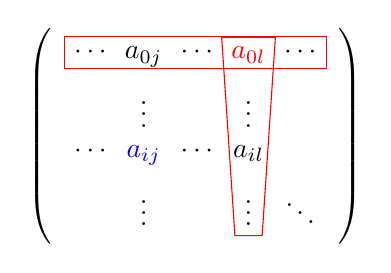
\begin{tikzpicture}
        \matrix [matrix of math nodes,left delimiter=(,right delimiter=)] (m)
        {
            \cdots & a_{0j} & \cdots & \color{red}a_{0l} &\cdots \\
            		 & \vdots &  & \vdots &  \\ 
			\cdots & \color{blue}a_{ij} & \cdots & a_{il}  & \\
			& \vdots &  & \vdots & \ddots \\
        };  
       \draw[color=red] (m-1-1.north west) -- (m-1-5.north east) -- (m-1-5.south east) -- (m-1-1.south west) -- (m-1-1.north west);
       \draw[color=red] (m-1-4.north west) -- (m-1-4.north east) -- (m-4-4.south east) -- (m-4-4.south west) -- (m-1-4.north west);
    \end{tikzpicture}


\subsection{Osservazioni sui programmi}
Cuda FloatMatrixClass: efficienza initializzazione curand dipende molto dalla scheda, su lara la cpu vince mentre su jacobi la gpu


\begin{figure}[ht!]
	\centering
	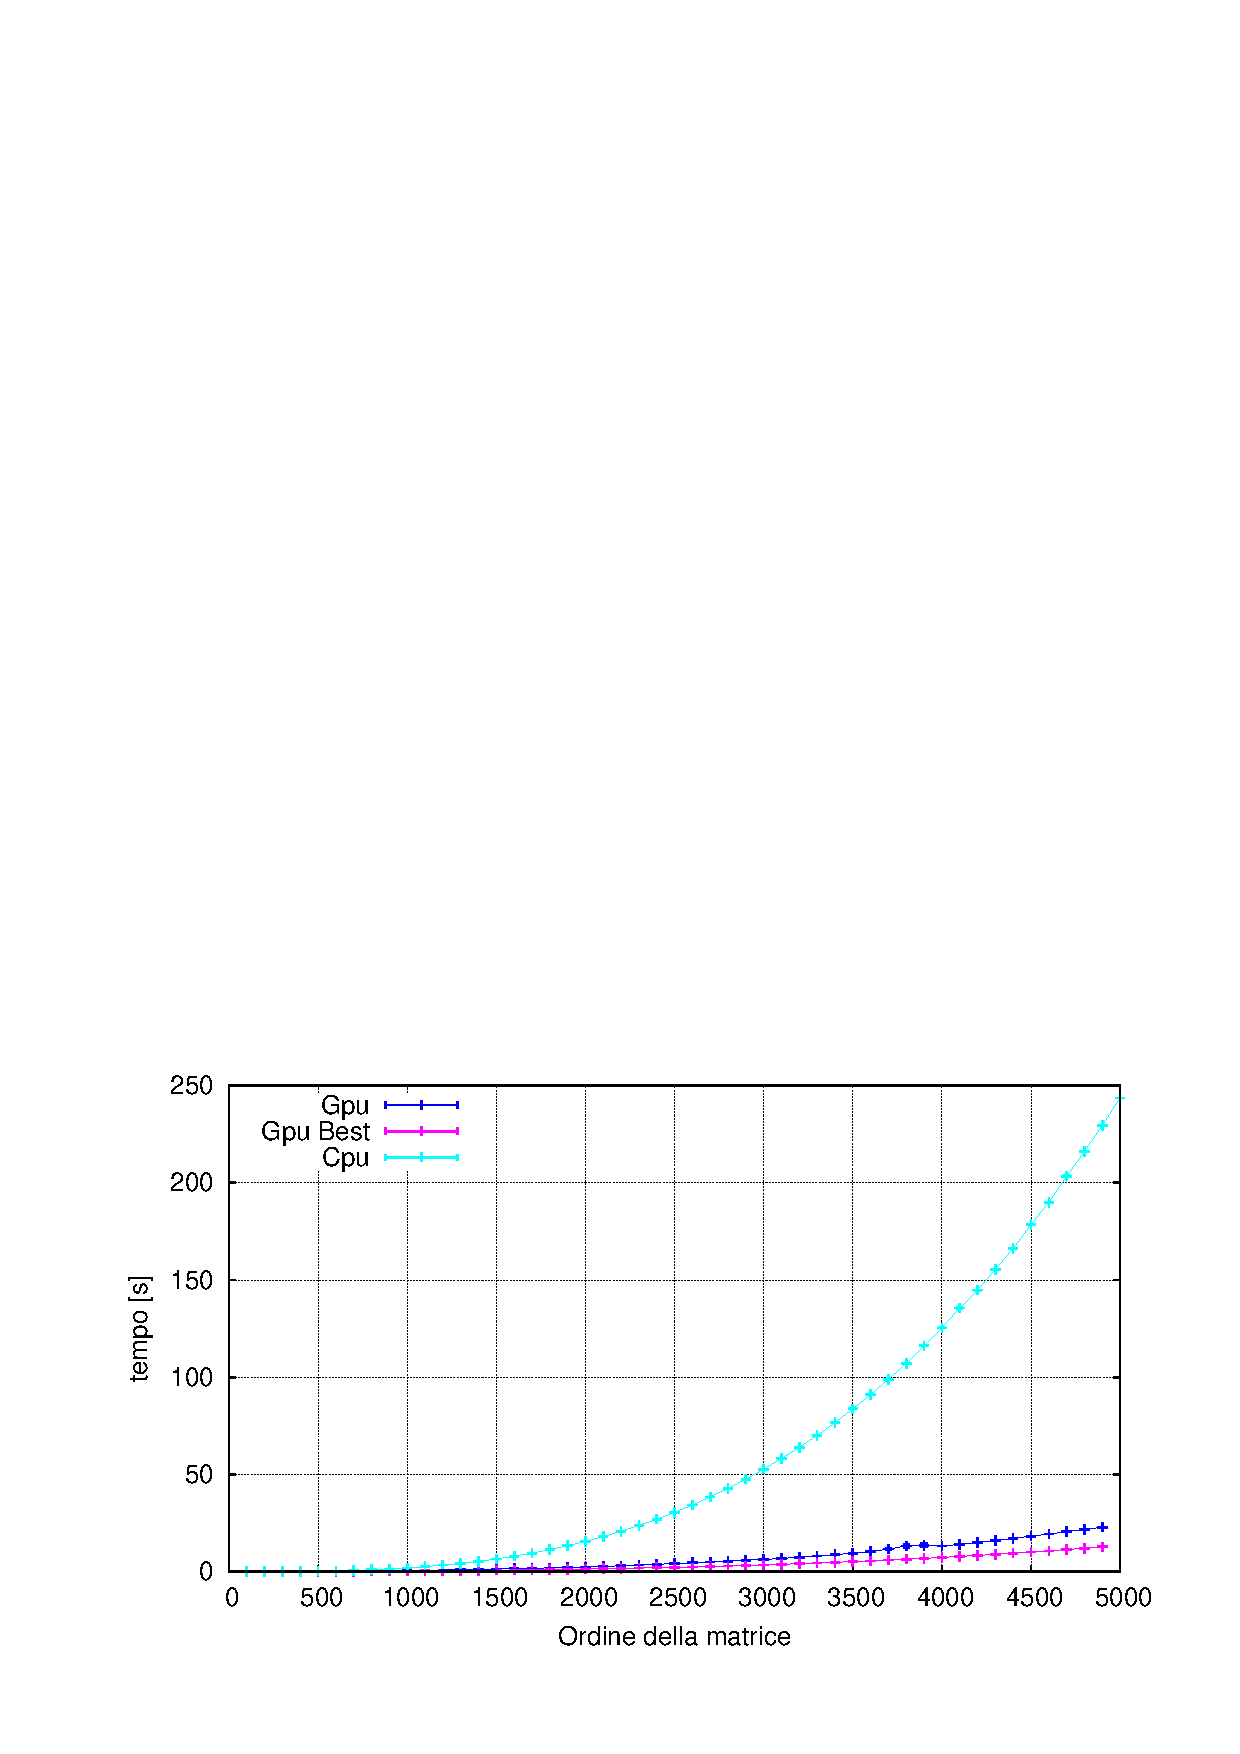
\includegraphics[width=180mm]{TimevsN.pdf}
	\caption{Confronto tempo d'esecuzione vs Taglia della matrice}
	\label{TimevsN}
\end{figure}

\begin{figure}[ht!]
	\centering
	\caption{Confronto tempo d'esecuzione vs Taglia della matrice (zoom)}
	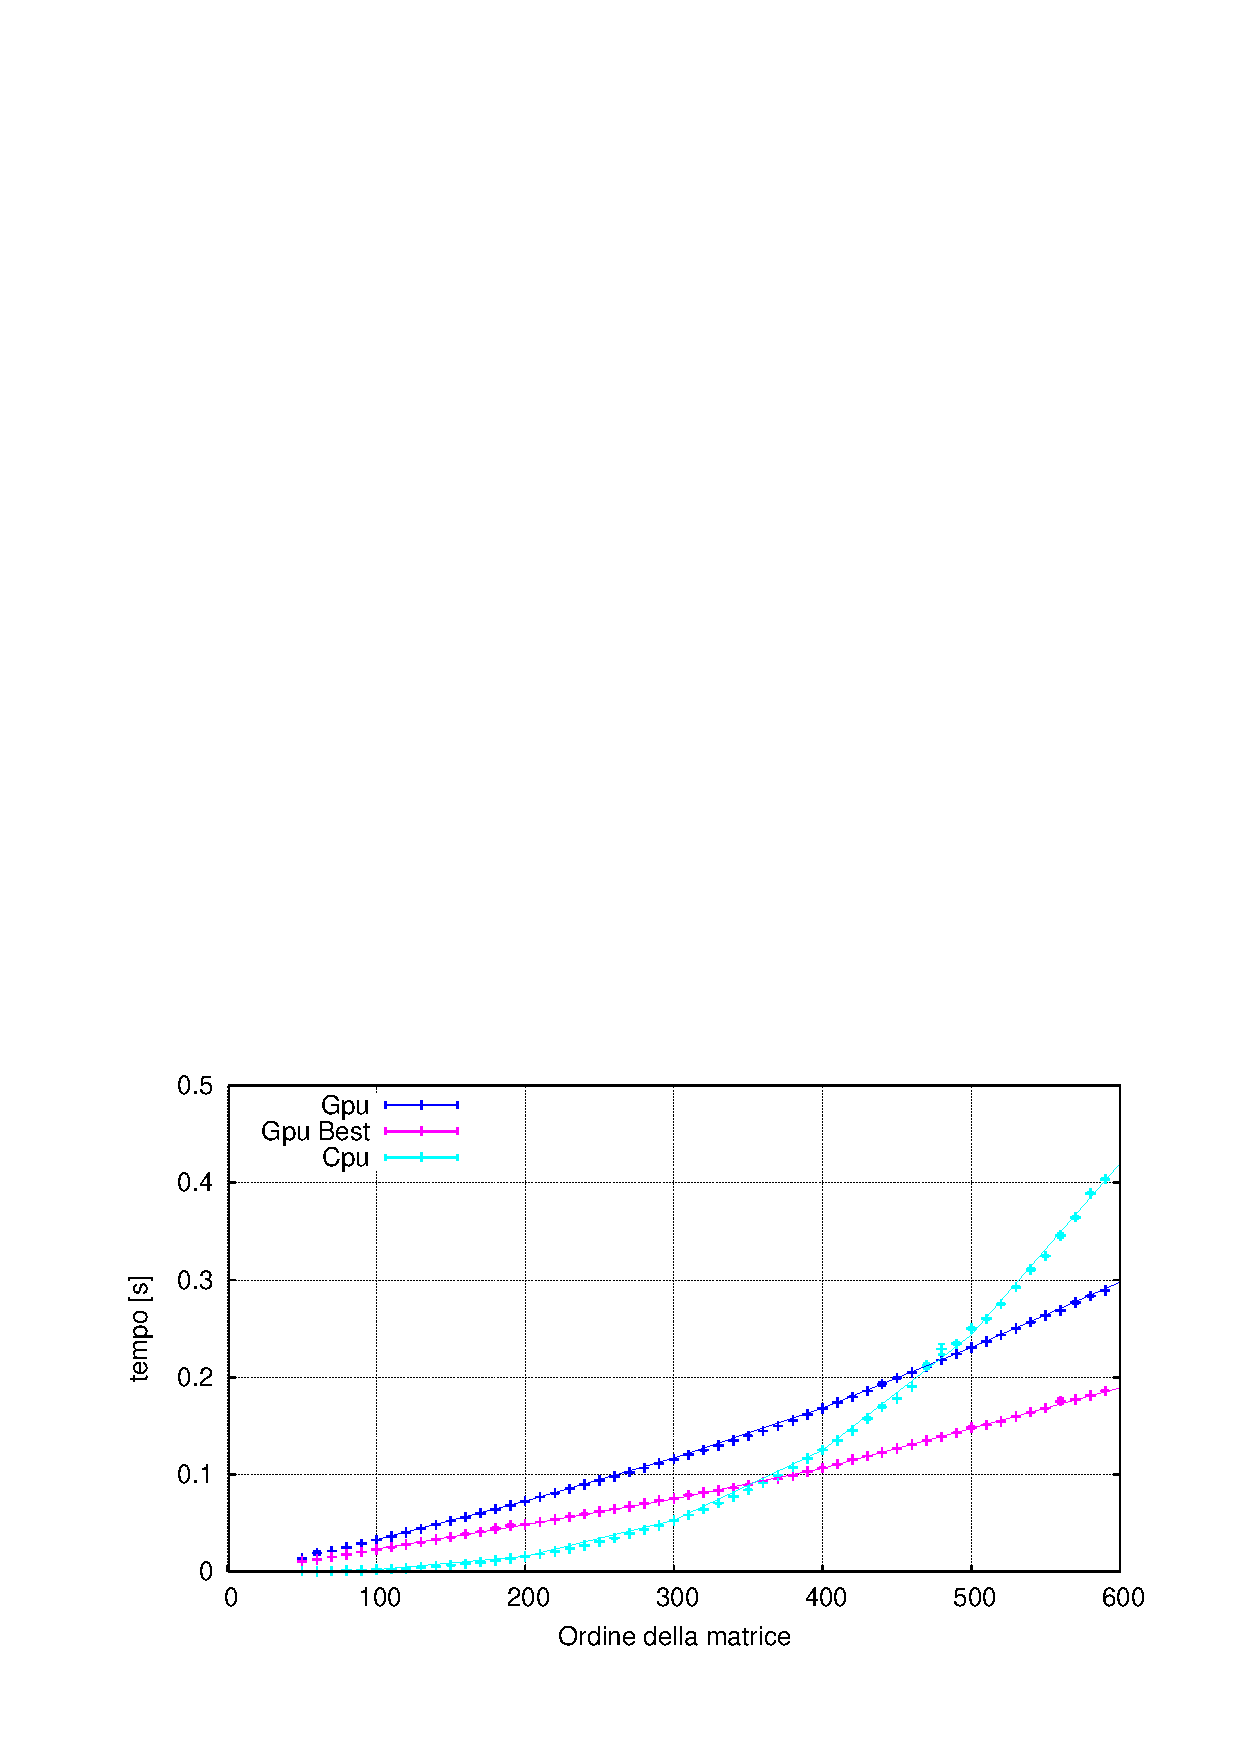
\includegraphics[width=180mm]{TimevsN_Zoom.pdf}
	\label{Zoom}
\end{figure}

\newpage 
\begin{thebibliography}{99}
\bibitem{Carroll} \textit{Dodgson .C L.} Condensation of Determinants \textit{Proceedings of the R. Society London 1866 }

\bibitem{arx:SalemSaid} \textit{Abdelmalek Salem, Kouachi Said.} Condensation of Determinants \textbf{http://arxiv.org/abs/0712.0822}

\bibitem{arx:MorenoHaque} \textit{Sardar Anisul Haque, Marc Moreno Maza.} Determinant Computation on the GPU using the Condensation Method \textbf{http://hgpu.org/?p=7012}


\end{thebibliography}
\end{document}